\section{Museum's role in society}
In the recommendation letter report \emph{“Museums in the society - trust, things and time”} the standing committee of Cultural Affairs present the overall political direction for Norwegian museum policy towards the year 2050. It is established that Norwegian museum institutions take aim at being an expression of both historical and current developments in society. And that museum institutions play an important role in our own time’s understanding of ourselves - both who we have been, who we are, and who we want to be \autocite[p. 7]{melding23}. Modern museum operations is aimed to actively turn to the general public, with the objective to build and share knowledge, increase enlightenment and cultivate cultural capital.

\begin{figure}[H]
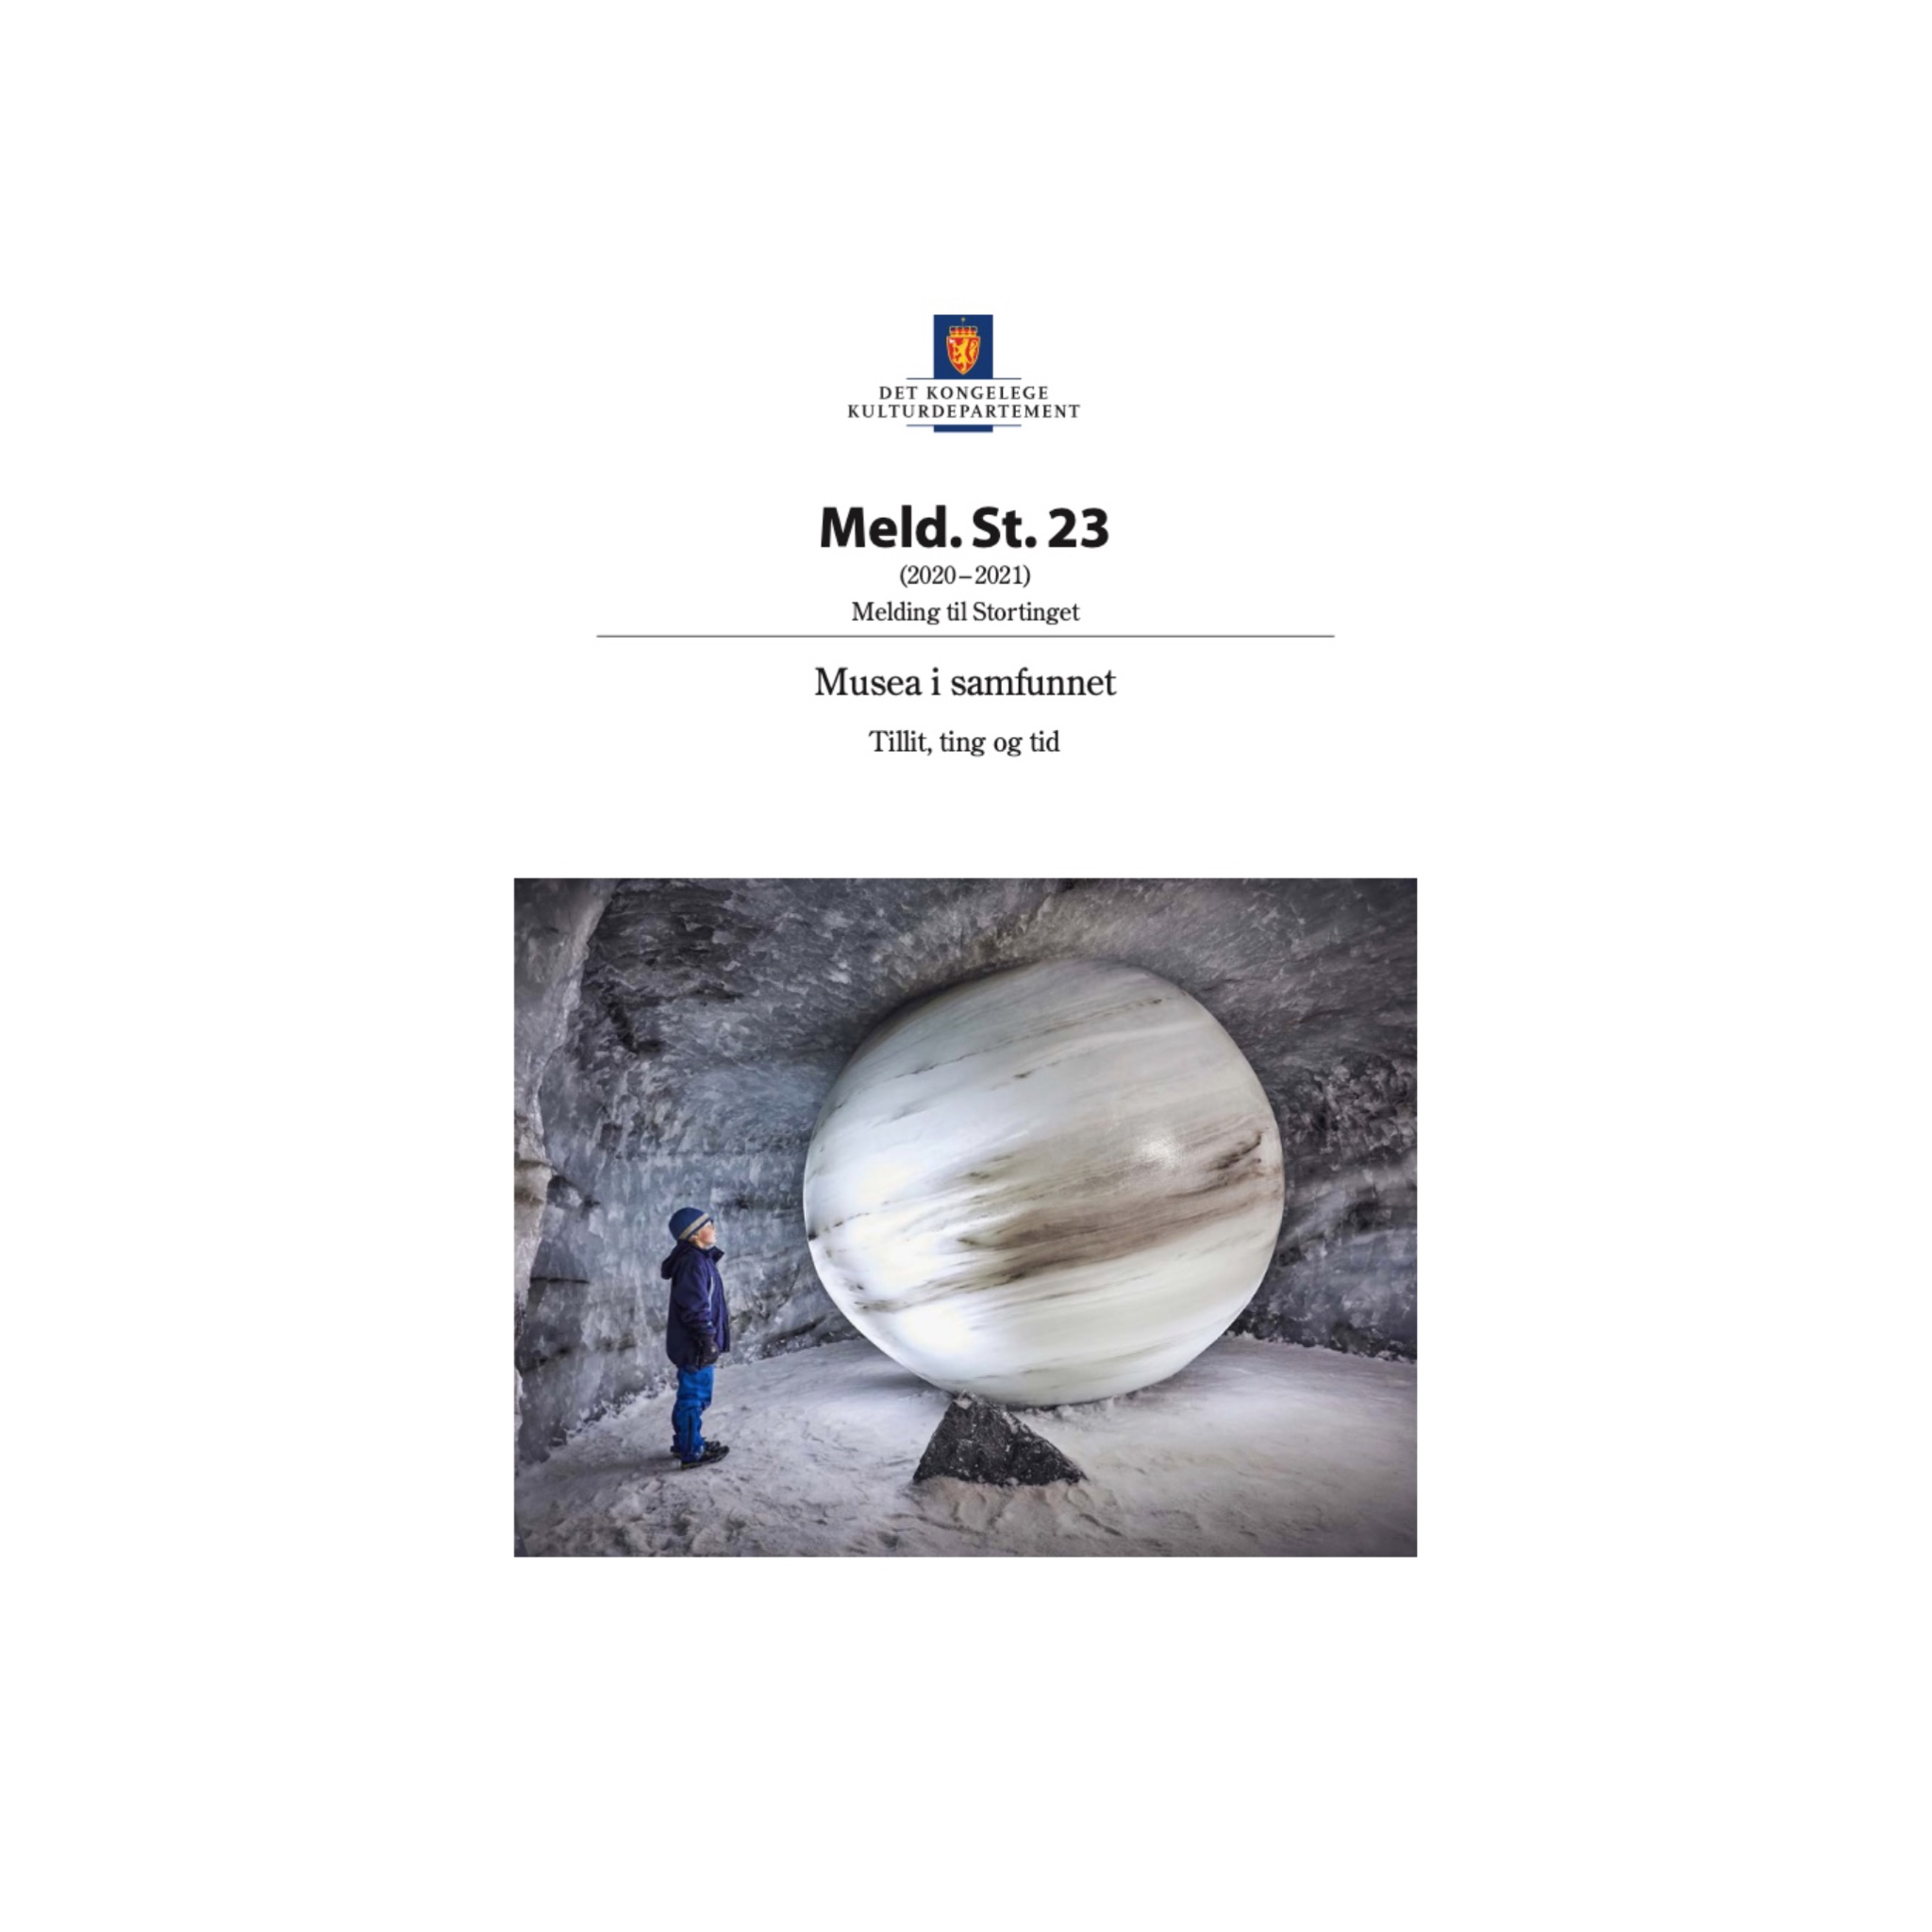
\includegraphics[width=11cm]{pictures/stortingsmelding.jpg}
\caption{The recommendation letter report Meld.St.23 \emph{“Museums in the society - trust, things and time"}}
\centering 
\end{figure}

Where the early museum institutions first and foremost were accessible to a small number of privileged class members, it is now expected that museums purposefully reach out to be open and accessible to all residents and age groups \autocite[p. 14]{melding23}. In Norway, museums are increasingly understood as being both a knowledge- and a social institution, where dissemination and exhibition practice is curated accordingly. At the same time, museums have emerged as an alternative learning arena for school children, first in regards of history teaching, but later in many other subject areas as well. In a society where polarization and public debate is intensifying, arenas that have the public's confidence in being able to nuance and disseminate different perspectives are needed \autocite[p. 7]{melding23}. There is a saying among historians that \emph{"the past teaches us about the present"}. Because history gives us the tools to analyze and explain problems in the past, it positions us to see patterns that might otherwise be invisible in the present – thus providing a crucial perspective for understanding (and solving!) current and future problems \autocite{UW_website}. Being an institution of knowledge, museums have the power to both define and showcase relevant historical events as a perspective to inform present societal issues and debates. 

%\emph{Jobbe litt med overgang her for å passe ordentlig inn! Få inn noe eget/ personlig motivasjon kanskje?}


\section{Research Question/ Framing}
The aim of this study is to gain insight to try answer how one can design interactive meaningful experiences in a museum space that addresses sustainability. To understand this, several installations have been analysed as a way to synthesise (or objectifying?) \emph{meaningfulness} as a quality that you can design for. Meaningfulness is defined/understood as (...), but this thesis fills a gap where the term is explored through a museum context, adding to existing literature on future museum design by using sustainability as a topic representing a contemporary discourse addressed in museum spaces.

\begin{itemize}
    \item \textbf{Main RQ:} How can one design meaningful interactive experiences in a museum space that addresses sustainability?
    \item answered by: \emph{(Sub-RQ):} synthesising (or objectifying?) meaningfulness as a quality that you can design for in a museum.
    \item through: \emph{(Sub-RQ):} finding/identifying dialogic relations between visitor and installation.
\end{itemize}


\section{Scientific contribution}
The thesis investigates how interactivity can support visitors meaning-making in a museum space. The hypothesis is that an interactive installation or experience have the potential to reinforce the message conveyed in a manner that give rise to thought-provoking or significant reflections that last long after the museum visit. Something which also encompass the power to deliberately stimulate visitors lifestyle choices or actions after the museum visit, in compliance with the museums agenda and vision. Special attention has been given to museums that aims to encourage social action, like climate consciousness or climate action.

The nature of the contributions:
\begin{itemize}
    \item theoretical contribution: analytical tool
    \item contribution to field (?): patterns
\end{itemize}

\section{About the structure of thesis}
What is important that the reader know before we dive into Background \& Theoretical influences?

This thesis is atypically structured because of the methodological nature (RtD) and therefore coming-together of the thesis. The thesis consist of four parts; Introduction, Background \& Theoretical influences, The Project, and Concluding. This thesis are quite picture-heavy, and if not referenced else-wise, all pictures are taken by me or my research buddies during the fieldwork of this thesis.